\section{Architecture}
\label{sec:architecture}

In this section we first clarify the \emph{application stack} we are assuming the SaaS application to have. Then we explain the different architectural approaches to implement versioning of SaaS, with \emph{multi-instance} as well as \emph{shared-instance} on the different application stack layers.

One important assumption we make for versioning is, that each tenant and therefore also all users of a tenant use the same version at the same time. Practially this means that each tenant has a dedicated migration point in which they decide to switch their version. This switch affects all their users at the same time. Users aren't allowed to individually choose their version.

\subsection{Application Stack}

\begin{wrapfigure}{r}{0.4\textwidth}
\centering
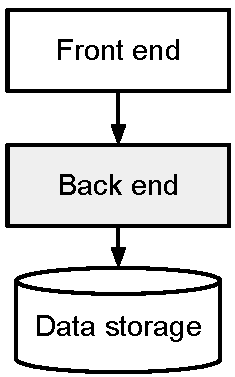
\includegraphics[width=0.3\textwidth]{stack.pdf}
\caption{Simplified Application Stack}
\label{fig:stack}
\end{wrapfigure}

To understand the architecture better, we first want to look at the SaaS application stack as displayed in Figure~\ref{fig:stack}. We derived this stack from our experience with developing SaaS ourselves as well as stacks we have seen in related papers (TODO references).

We assume a separation between the front-end, back-end and database layer. The front-end layer is mainly concerned with the user interface. In a SaaS it will usually be delivered to the user's browser within a request/response cycle. The back-end layer is concerned with the application and business logic. It takes requests from the front-end layer and accordingly communicated with the database layer. The front-end and back-end layers are stateless, because all state is kept in the database layer.

To focus our research, we omitted some details of the stack. First we did were not concerned with caching as well as load balancing. Furthermore we omitted how user management is done, especially with regards to authentication.

\subsection{Multi-Instance}

Not multi-tenant in itself, but usually the most inuitive way to provide saas. good if not too many clients.

multi-tenancy using multi-instance
though this seems simple from an architectual perspective
bad consolidation factor
high maintenance cost as operation complexity increases with the number of tenants
not the spirit of SaaS

\subsection{Shared-Instance}

\subsubsection{Frontend}
  Web application
  tight coupling between backend and frontend
  simultaneously versioned
  versioning concern in backend

  API consumers (e.g. native apps)
  loose coupling between backend and frontend
  backend needs to provide different versions of API
  api consumers choose version

  Frontend API Versioning
    In URL:
      http://api.com/v1/resource.json?version=1
    Accept Header:
      Accept: application/json+v1
    Application Flag:

\subsubsection{Backend}
\paragraph{Shared-Instance 1:1}
geiles diagram

a product ver = code rev


Pro
Versioning is external to application code

Contra
heterogeneous deployment
worse consolidation factor
intelligent routing layer needed
forking of code base makes security patches difficult to apply



\paragraph{Shared-Instance 1:n}
geiles diagram


version choice is on app server


Pro
good consolidation
homogenous deployment
more flexibility: fine grained feature selection

Contra
increased code complexity
abandoning old versions needs cleanup



inside of code base are many version checks "if version == 1.4 ..."
more flexibility in choosing version, maybe not choose version but choose only features

high cost for abandoning old version to clean code base

\lstset{language=Ruby, caption=code snippet, label=code}
\begin{lstlisting}
  if(user.has_version?):
    do_something()
  end
\end{lstlisting}

\subsubsection{Database}

\paragraph{Different versions share same schema}
db is version agnostic

\paragraph{Different versions need separate schemas}
How to version schemas?

  Database needs to support several schemas for a table at the same time

  No DBMs supporting this is known to us

  Thus versioning has to happen in the backend

  \paragraph{Different tables for each schema}
  \lstset{language=SQL, caption=sql, label=sql}
  \begin{lstlisting}
    create table users_v1;
    create table users_v2;
    create table users_v3;
  \end{lstlisting}

  Pro:
  Works well if not too many versions

  Con:
  Messy design if many versions


  \paragraph{Pivot tables}

  bild von "An Elastic Multi-tenant Database Schema for Software as a Service"

  reduce dbms more to a key value store
  as used with salesforce

\paragraph{Migration of data}
  version is chosen per tenant
  data migrations need time
  data migrations might need downtime
  on-the-fly migrations possible

